\documentclass[twoside,11pt]{article}

% ? Specify used packages
\usepackage{graphicx}        %  Use this one for final production.
% \usepackage[draft]{graphicx} %  Use this one for drafting.
% ? End of specify used packages

\pagestyle{myheadings}

% -----------------------------------------------------------------------------
% ? Document identification
% Fixed part
\newcommand{\stardoccategory}  {STARLINK User Note}
\newcommand{\stardocinitials}  {SUN}
\newcommand{\stardocsource}    {sun\stardocnumber}

% Variable part - replace [xxx] as appropriate.
\newcommand{\stardocnumber}    {237.1}
\newcommand{\stardocauthors}   {A.~Allan}
\newcommand{\stardocdate}      {2nd January 2001}
\newcommand{\stardoctitle}     {DATACUBE --- An IFS datacube manipulation package}
\newcommand{\stardocversion}   {version 1.0}
\newcommand{\stardocmanual}    {User's Manual}
\newcommand{\stardocabstract}  {  
\htmlref{DATACUBE}{DATACUBE} is a package which includes the IFU Data Product Cookbook (\xref{SC/16}{sc16}{}), a small number of applications used for AXIS and WCS manipulation, and a collection of example shell and IDL scripts for IFS data cube manipulation.
}

% ? End of document identification
% -----------------------------------------------------------------------------

% +
%  Name:
%     sc.tex
%
%  Purpose:
%     Template for Starlink Cookbook (SC) documents.
%     Refer to SUN/199
%
%  Authors:
%     AJC: A.J.Chipperfield (Starlink, RAL)
%     BLY: M.J.Bly (Starlink, RAL)
%
%  History:
%     16-JUN-1997 (BLY):
%        Original, based on SUN/SG templates.
%     {Add further history here}
%
% -

\newcommand{\stardocname}{\stardocinitials /\stardocnumber}
\markboth{\stardocname}{\stardocname}
\setlength{\textwidth}{160mm}
\setlength{\textheight}{230mm}
\setlength{\topmargin}{-2mm}
\setlength{\oddsidemargin}{0mm}
\setlength{\evensidemargin}{0mm}
\setlength{\parindent}{0mm}
\setlength{\parskip}{\medskipamount}
\setlength{\unitlength}{1mm}

% -----------------------------------------------------------------------------
%  Hypertext definitions.
%  ======================
%  These are used by the LaTeX2HTML translator in conjunction with star2html.

%  Comment.sty: version 2.0, 19 June 1992
%  Selectively in/exclude pieces of text.
%
%  Author
%    Victor Eijkhout                                      <eijkhout@cs.utk.edu>
%    Department of Computer Science
%    University Tennessee at Knoxville
%    104 Ayres Hall
%    Knoxville, TN 37996
%    USA

%  Do not remove the %\begin{rawtex} and %\end{rawtex} lines (used by 
%  star2html to signify raw TeX that latex2html cannot process).
%\begin{rawtex}
\makeatletter
\def\makeinnocent#1{\catcode`#1=12 }
\def\csarg#1#2{\expandafter#1\csname#2\endcsname}

\def\ThrowAwayComment#1{\begingroup
    \def\CurrentComment{#1}%
    \let\do\makeinnocent \dospecials
    \makeinnocent\^^L% and whatever other special cases
    \endlinechar`\^^M \catcode`\^^M=12 \xComment}
{\catcode`\^^M=12 \endlinechar=-1 %
 \gdef\xComment#1^^M{\def\test{#1}
      \csarg\ifx{PlainEnd\CurrentComment Test}\test
          \let\html@next\endgroup
      \else \csarg\ifx{LaLaEnd\CurrentComment Test}\test
            \edef\html@next{\endgroup\noexpand\end{\CurrentComment}}
      \else \let\html@next\xComment
      \fi \fi \html@next}
}
\makeatother

\def\includecomment
 #1{\expandafter\def\csname#1\endcsname{}%
    \expandafter\def\csname end#1\endcsname{}}
\def\excludecomment
 #1{\expandafter\def\csname#1\endcsname{\ThrowAwayComment{#1}}%
    {\escapechar=-1\relax
     \csarg\xdef{PlainEnd#1Test}{\string\\end#1}%
     \csarg\xdef{LaLaEnd#1Test}{\string\\end\string\{#1\string\}}%
    }}

%  Define environments that ignore their contents.
\excludecomment{comment}
\excludecomment{rawhtml}
\excludecomment{htmlonly}
%\end{rawtex}

%  Hypertext commands etc. This is a condensed version of the html.sty
%  file supplied with LaTeX2HTML by: Nikos Drakos <nikos@cbl.leeds.ac.uk> &
%  Jelle van Zeijl <jvzeijl@isou17.estec.esa.nl>. The LaTeX2HTML documentation
%  should be consulted about all commands (and the environments defined above)
%  except \xref and \xlabel which are Starlink specific.

\newcommand{\htmladdnormallinkfoot}[2]{#1\footnote{#2}}
\newcommand{\htmladdnormallink}[2]{#1}
\newcommand{\htmladdimg}[1]{}
\newenvironment{latexonly}{}{}
\newcommand{\hyperref}[4]{#2\ref{#4}#3}
\newcommand{\htmlref}[2]{#1}
\newcommand{\htmlimage}[1]{}
\newcommand{\htmladdtonavigation}[1]{}

%  Starlink cross-references and labels.
\newcommand{\xref}[3]{#1}
\newcommand{\xlabel}[1]{}

%  LaTeX2HTML symbol.
\newcommand{\latextohtml}{{\bf LaTeX}{2}{\tt{HTML}}}

%  Define command to re-centre underscore for Latex and leave as normal
%  for HTML (severe problems with \_ in tabbing environments and \_\_
%  generally otherwise).
\newcommand{\latex}[1]{#1}
\newcommand{\setunderscore}{\renewcommand{\_}{{\tt\symbol{95}}}}
\latex{\setunderscore}

%  Redefine the \tableofcontents command. This procrastination is necessary 
%  to stop the automatic creation of a second table of contents page
%  by latex2html.
\newcommand{\latexonlytoc}[0]{\tableofcontents}

% Figure environment. Defined for latex2html. #1 is postscript file
% #2 the qualifiers, #3 the gif file, #4 the label, #5 the caption.
\newcommand{\myfig} [5] {
  \begin{figure}
    \centering\includegraphics[#2]{#1}
    \typeout{#1 inserted on page \arabic{page}}
    \caption{\label{#4}#5}
  \end{figure}
  }
\begin{htmlonly}
  \newcommand{\myfig}[5]{
    \label{#4} \htmladdimg{#3}\\
    Figure: #5\\
    }
\end{htmlonly}

% -----------------------------------------------------------------------------
%  Debugging.
%  =========
%  Remove % on the following to debug links in the HTML version using Latex.

% \newcommand{\hotlink}[2]{\fbox{\begin{tabular}[t]{@{}c@{}}#1\\\hline{\footnotesize #2}\end{tabular}}}
% \renewcommand{\htmladdnormallinkfoot}[2]{\hotlink{#1}{#2}}
% \renewcommand{\htmladdnormallink}[2]{\hotlink{#1}{#2}}
% \renewcommand{\hyperref}[4]{\hotlink{#1}{\S\ref{#4}}}
% \renewcommand{\htmlref}[2]{\hotlink{#1}{\S\ref{#2}}}
% \renewcommand{\xref}[3]{\hotlink{#1}{#2 -- #3}}
% -----------------------------------------------------------------------------
% ? Document specific \newcommand or \newenvironment commands.
% ? End of document specific commands
% -----------------------------------------------------------------------------
%  Title Page.
%  ===========
\renewcommand{\thepage}{\roman{page}}
\begin{document}
\thispagestyle{empty}

%  Latex document header.
%  ======================
\begin{latexonly}
   CCLRC / {\sc Rutherford Appleton Laboratory} \hfill {\bf \stardocname}\\
   {\large Particle Physics \& Astronomy Research Council}\\
   {\large Starlink Project\\}
   {\large \stardoccategory\ \stardocnumber}
   \begin{flushright}
   \stardocauthors\\
   \stardocdate
   \end{flushright}
   \vspace{-4mm}
   \rule{\textwidth}{0.5mm}
   \vspace{5mm}
   \begin{center}
   {\Huge\bf  \stardoctitle \\ [2.5ex]}
   \end{center}
   \vspace{5mm}

% ? Add picture here if required for the LaTeX version.
%   e.g. \includegraphics[scale=0.3]{filename.ps}
   \begin{center}
   \includegraphics[scale=0.6]{sun237_cover.eps}
   \end{center}
% ? End of picture

% ? Heading for abstract if used.
   \vspace{5mm}
   \begin{center}
      {\Large\bf Abstract}
   \end{center}
% ? End of heading for abstract.
\end{latexonly}

%  HTML documentation header.
%  ==========================
\begin{htmlonly}
   \xlabel{}
   \begin{rawhtml} <H1> \end{rawhtml}
      \stardoctitle\\
      \stardocversion\\
      \stardocmanual
   \begin{rawhtml} </H1> \end{rawhtml}

% ? Add picture here if required for the hypertext version.
%   e.g. \includegraphics[scale=0.7]{filename.ps}
   \htmladdimg{sun237_cover.gif}

% ? End of picture

   \begin{rawhtml} <P> <I> \end{rawhtml}
   \stardoccategory \stardocnumber \\
   \stardocauthors \\
   \stardocdate
   \begin{rawhtml} </I> </P> <H3> \end{rawhtml}
      \htmladdnormallink{CCLRC}{http://www.cclrc.ac.uk} /
      \htmladdnormallink{Rutherford Appleton Laboratory}
                        {http://www.cclrc.ac.uk/ral} \\
      \htmladdnormallink{Particle Physics \& Astronomy Research Council}
                        {http://www.pparc.ac.uk} \\
   \begin{rawhtml} </H3> <H2> \end{rawhtml}
      \htmladdnormallink{Starlink Project}{http://star-www.rl.ac.uk/}
   \begin{rawhtml} </H2> \end{rawhtml}
   \htmladdnormallink{\htmladdimg{source.gif} Retrieve hardcopy}
      {http://star-www.rl.ac.uk/cgi-bin/hcserver?\stardocsource}\\

%  HTML document table of contents. 
%  ================================
%  Add table of contents header and a navigation button to return to this 
%  point in the document (this should always go before the abstract \section). 
  \label{stardoccontents}
  \begin{rawhtml} 
    <HR>
    <H2>Contents</H2>
  \end{rawhtml}
  \renewcommand{\latexonlytoc}[0]{}
%  \htmladdtonavigation{\htmlref{\htmladdimg{sc15_cover.gif}}
%        {stardoccontents}}

% ? New section for abstract if used.
  \section{\xlabel{abstract}Abstract}
% ? End of new section for abstract
\end{htmlonly}

% -----------------------------------------------------------------------------
% ? Document Abstract. (if used)
%  ==================
\stardocabstract
% ? End of document abstract
% -----------------------------------------------------------------------------
% ? Latex document Table of Contents (if used).
%  ===========================================
 \newpage
 \vspace{3cm}

 \subsection*{Revision history}

 \begin{enumerate}
   \item 9th November 2000; Version 0.1 Original version (AA) 
   \item 30th December 2000; Version 0.2 Auto-generated code prologs (AA)
   \item 2nd January 2001; Version 1.0 Release version (AA)

 \end{enumerate}

 \vspace{10cm}
 \copyright \underline{1999-2001} Starlink, CCLRC

 \cleardoublepage
 \begin{latexonly}
   \setlength{\parskip}{0mm}
   \latexonlytoc

   \newpage
   \listoffigures
   %\listoftables

   \setlength{\parskip}{\medskipamount}
   \markright{\stardocname}
 \end{latexonly}
% ? End of Latex document table of contents
% -----------------------------------------------------------------------------

\cleardoublepage
\newpage
\renewcommand{\thepage}{\arabic{page}}
\setcounter{page}{1}

% The main text begins here.
% -----------------------------------------------------------------------------

\section{\xlabel{sun237_intro}The Datacube Package\label{sun237_intro}}

The backbone of the Datacube Package is the \xref{IFU Data Product Cookbook}{sc16}{} (SC/16). Accompanying this book is a collection of {\tt csh} scripts layered ontop of various pieces of the Starlink Software Collection (SSC), along with a couple of ADAM applications to manipulate WCS and AXIS extensions.

The C-Shell approach was a deliberate design decision which was made for two main reasons: Firstly, due to the still developing nature of the field it is difficult to pin down exactly visualisation tasks will be necessary, and the choice of {\tt csh} means that the existing scripts can be easily modified by the end user to do exactly the job required; Secondly, after examining the Starlink Software Collection (SSC) it was realised that a great deal of the functionality required to analyse IFU data already existed and it would be wasteful to re-invent the wheel by re-coding large chunks of software.

Some tasks once mature can, and should, be re-coded in FORTRAN or C, mainly for the speed and memory advantages that this will bring. For instance the \htmlref{{\tt velmap}}{velmap} script as implemented is rather slow and memory intensive, it seems likely that this will be the first candidate to be re-coded in a lower level language.

Hopefully, while I haven't managed to think of everything, there is enough ground work here so that the approach to solving your data visualisation or data cube manipulation problem is obvious, even if the package doesn't have a script or application to do exactly what you require. 

While this document contains the detailed descriptions of the A-tasks and shell scripts included with the package, the ``how to'' information  detailing their use can be found in \xref{SC/16}{sc16}{}.

I would welcome comments, criticisms, contributions and corrections to the package once people start to figure out what they want to do with this sort of data.  Comments can be sent either to me at \htmladdnormallink{aa@astro.ex.ac.uk}{mailto:aa@astro.ex.ac.uk} or to the Starlink software librarian \htmladdnormallink{ussc@star.rl.ac.uk}{mailto:ussc@star.rl.ac.uk}. 

\section{\xlabel{sun237_starting}Setting up the applications\label{sun237_starting}}

After sourcing the Starlink {\tt /star/etc/login} and {\tt /star/etc/cshrc} files the {\tt datacube} dcommand will make the datacube package commands and scripts available to you, the following message (or one much like it!) should appear

\small\begin{verbatim}
   % datacube
    
      DATACUBE applications are now available -- (Version 1.0)
       Support is available by emailing datacube@star.rl.ac.uk
    
           Type cubehelp for help on DATACUBE commands.
      Type 'showme sun237' to browse the hypertext documentation
      or 'showme sc16' to consult the IFU data product cookbook.
  
   %
\end{verbatim}\normalsize

at this point you can test whether the datacube package has been correctly installed by typing

\small\begin{verbatim}
   % datacube_test
\end{verbatim}\normalsize

which will run the test script for the package. If the script does not run correctly you should consult your Starlink system administrator.

It should be noted that there are a great many useful applications available in other Starlink packages that will assist you in dealing with your IFU data (see \xref{SC/16}{sc16}{} for details), so you may, at the very minimum, wish to setup the \xref{KAPPA}{sun95}{} applications with the {\tt kappa} command

\small\begin{verbatim}
   % kappa
 
        KAPPA commands are now available -- (Version 0.15-9)

        Type kaphelp for help on KAPPA commands.
        Type 'showme sun95' to browse the hypertext documentation.

        NOTE, several applications have had major changes made to their
        parameter lists. See the 'Release Notes' section of SUN/95 for
        details.
   %	
\end{verbatim}\normalsize

\section*{\xlabel{sun237_acks}Acknowledgments\label{sun237_acks}}

In compiling this document I have again depended heavily on the help of many people in the IFS community. However, special thanks should go to \htmladdnormallink{Rachel Johnston}{http://www.ast.cam.ac.uk/~raj/}, \htmladdnormallink{Jeremy Allington-Smith}{http://star-www.dur.ac.uk:80/~jra/}, \htmladdnormallink{James Turner}{mailto:J.E.H.Turner@durham.ac.uk} and \htmladdnormallink{Frank Valdes}{http://www.noao.edu/noao/scistaff/valdes.html} for their co-operation and contributions.

\newpage
\appendix
\section{DESCRIPTIONS OF INDIVIDUAL APPLICATIONS}
\label{sun237_appendix_descriptions}

% +
%  Name:
%     SST.TEX

%  Purpose:
%     Define LaTeX commands for laying out Starlink routine descriptions.

%  Language:
%     LaTeX

%  Type of Module:
%     LaTeX data file.

%  Description:
%     This file defines LaTeX commands which allow routine documentation
%     produced by the SST application PROLAT to be processed by LaTeX and
%     by LaTeX2html. The contents of this file should be included in the
%     source prior to any statements that make of the sst commnds.

%  Notes:
%     The commands defined in the style file html.sty provided with LaTeX2html
%     are used. These should either be made available by using the appropriate
%     sun.tex (with hypertext extensions) or by putting the file html.sty
%     on your TEXINPUTS path (and including the name as part of the
%     documentstyle declaration).

%  Authors:
%     RFWS: R.F. Warren-Smith (STARLINK)
%     PDRAPER: P.W. Draper (Starlink - Durham University)

%  History:
%     10-SEP-1990 (RFWS):
%        Original version.
%     10-SEP-1990 (RFWS):
%        Added the implementation status section.
%     12-SEP-1990 (RFWS):
%        Added support for the usage section and adjusted various spacings.
%     8-DEC-1994 (PDRAPER):
%        Added support for simplified formatting using LaTeX2html.
%     {enter_further_changes_here}

%  Bugs:
%     {note_any_bugs_here}

% -

%  Define length variables.
\newlength{\sstbannerlength}
\newlength{\sstcaptionlength}
\newlength{\sstexampleslength}
\newlength{\sstexampleswidth}

%  Define a \tt font of the required size.
\newfont{\ssttt}{cmtt10 scaled 1095}

%  Define a command to produce a routine header, including its name,
%  a purpose description and the rest of the routine's documentation.
\newcommand{\sstroutine}[3]{
   \goodbreak
   \rule{\textwidth}{0.5mm}
   \vspace{-7ex}
   \newline
   \settowidth{\sstbannerlength}{{\Large {\bf #1}}}
   \setlength{\sstcaptionlength}{\textwidth}
   \setlength{\sstexampleslength}{\textwidth}
   \addtolength{\sstbannerlength}{0.5em}
   \addtolength{\sstcaptionlength}{-2.0\sstbannerlength}
   \addtolength{\sstcaptionlength}{-5.0pt}
   \settowidth{\sstexampleswidth}{{\bf Examples:}}
   \addtolength{\sstexampleslength}{-\sstexampleswidth}
   \parbox[t]{\sstbannerlength}{\flushleft{\Large {\bf #1}}}
   \parbox[t]{\sstcaptionlength}{\center{\Large #2}}
   \parbox[t]{\sstbannerlength}{\flushright{\Large {\bf #1}}}
   \begin{description}
      #3
   \end{description}
}

%  Format the description section.
\newcommand{\sstdescription}[1]{\item[Description:] #1}

%  Format the usage section.
\newcommand{\sstusage}[1]{\item[Usage:] \mbox{} \\[1.3ex] {\ssttt #1}}


%  Format the invocation section.
\newcommand{\sstinvocation}[1]{\item[Invocation:]\hspace{0.4em}{\tt #1}}

%  Format the arguments section.
\newcommand{\sstarguments}[1]{
   \item[Arguments:] \mbox{} \\
   \vspace{-3.5ex}
   \begin{description}
      #1
   \end{description}
}

%  Format the returned value section (for a function).
\newcommand{\sstreturnedvalue}[1]{
   \item[Returned Value:] \mbox{} \\
   \vspace{-3.5ex}
   \begin{description}
      #1
   \end{description}
}

%  Format the parameters section (for an application).
\newcommand{\sstparameters}[1]{
   \item[Parameters:] \mbox{} \\
   \vspace{-3.5ex}
   \begin{description}
      #1
   \end{description}
}

%  Format the examples section.
\newcommand{\sstexamples}[1]{
   \item[Examples:] \mbox{} \\
   \vspace{-3.5ex}
   \begin{description}
      #1
   \end{description}
}

%  Define the format of a subsection in a normal section.
\newcommand{\sstsubsection}[1]{ \item[{#1}] \mbox{} \\}

%  Define the format of a subsection in the examples section.
\newcommand{\sstexamplesubsection}[2]{\sloppy
\item[\parbox{\sstexampleslength}{\ssttt #1}] \mbox{} \\ #2 }

%  Format the notes section.
\newcommand{\sstnotes}[1]{\item[Notes:] \mbox{} \\[1.3ex] #1}

%  Provide a general-purpose format for additional (DIY) sections.
\newcommand{\sstdiytopic}[2]{\item[{\hspace{-0.35em}#1\hspace{-0.35em}:}] \mbox{} \\[1.3ex] #2}

%  Format the implementation status section.
\newcommand{\sstimplementationstatus}[1]{
   \item[{Implementation Status:}] \mbox{} \\[1.3ex] #1}

%  Format the bugs section.
\newcommand{\sstbugs}[1]{\item[Bugs:] #1}

%  Format a list of items while in paragraph mode.
\newcommand{\sstitemlist}[1]{
  \mbox{} \\
  \vspace{-3.5ex}
  \begin{itemize}
     #1
  \end{itemize}
}

%  Define the format of an item.
\newcommand{\sstitem}{\item}

%  Now define html equivalents of those already set. These are used by
%  latex2html and are defined in the html.sty files.
\begin{htmlonly}

%  Re-define \ssttt.
   \newcommand{\ssttt}{\tt}

%  sstroutine.
   \renewcommand{\sstroutine}[3]{
      \subsection{#1\xlabel{#1}-\label{#1}#2}
      \begin{description}
         #3
      \end{description}
   }

%  sstdescription
   \renewcommand{\sstdescription}[1]{\item[Description:]
      \begin{description}
         #1
      \end{description}
   }

%  sstusage
   \renewcommand{\sstusage}[1]{\item[Usage:]
      \begin{description}
         {\ssttt #1}
      \end{description}
   }

%  sstinvocation
   \renewcommand{\sstinvocation}[1]{\item[Invocation:]
      \begin{description}
         {\ssttt #1}
      \end{description}
   }

%  sstarguments
   \renewcommand{\sstarguments}[1]{
      \item[Arguments:]
      \begin{description}
         #1
      \end{description}
   }

%  sstreturnedvalue
   \renewcommand{\sstreturnedvalue}[1]{
      \item[Returned Value:]
      \begin{description}
         #1
      \end{description}
   }

%  sstparameters
   \renewcommand{\sstparameters}[1]{
      \item[Parameters:]
      \begin{description}
         #1
      \end{description}
   }

%  sstexamples
   \renewcommand{\sstexamples}[1]{
      \item[Examples:]
      \begin{description}
         #1
      \end{description}
   }

%  sstsubsection
   \renewcommand{\sstsubsection}[1]{\item[{#1}]}

%  sstexamplesubsection
   \renewcommand{\sstexamplesubsection}[2]{\item[{\ssttt #1}] \\ #2}

%  sstnotes
   \renewcommand{\sstnotes}[1]{\item[Notes:]
      \begin{description}
         #1
      \end{description}
   }

%  sstdiytopic
   \renewcommand{\sstdiytopic}[2]{\item[{#1}]
      \begin{description}
         #2
      \end{description}
   }

%  sstimplementationstatus
   \renewcommand{\sstimplementationstatus}[1]{\item[Implementation Status:]
      \begin{description}
         #1
      \end{description}
   }

%  sstitemlist
   \newcommand{\sstitemlist}[1]{
      \begin{itemize}
         #1
      \end{itemize}
   }
\end{htmlonly}

%  End of "sst.tex" layout definitions.
% .
% @(#)sst.tex   1.4   95/06/06 11:46:41   96/07/05 10:28:17

\sstroutine{
   compare
}{
   Comparison of multiple extracted spectra from a 3D IFU NDF
}{
   \sstdescription{
      This shell script sits onto of a collection of A-tasks from the KAPPA
      FIGARO and DATACUBE packages. It reads a 3D IFU NDF datacube as input
      and presents the user with a white light image of the cube. The user
      can then select and x,y position using the cursor. The script will
      extract and display this spectra next to the white light image. The
      user can then select another x,y position using the cursor and the
      script will display this spectra as well, allowing comparison of the two.
   }
   \sstusage{
      compare
   }
   \sstdiytopic{
      Copyright
   }{
      Copyright (C) 2000 Central Laboratory of the Research Councils
   }
}
\newpage
\sstroutine{
   COPYAXIS
}{
   Copies an AXIS extension into an NDF from the information present in
   another NDF
}{
   \sstdescription{
      Simple application designed to be run from inside a user written
      script or from the command line, it will build an AXIS extension
      for a specified NDF from the information present in an NDF of identical
      dimensionality and bounds.
   }
   \sstusage{
      copyaxis in=file like=template
   }
   \sstparameters{
      \sstsubsection{
         IN = \_NDF (Read \& Write)
      }{
         The NDF to be modified
      }
      \sstsubsection{
         LIKE = \_NDF (Read)
      }{
         The template NDF.
      }
   }
   \sstexamples{
      \sstexamplesubsection{
         copyaxis in=smirfp0 like=smirfsp1
      }{
         Copies the AXIS structure from the file smirfsp1 to smirfsp0
      }
   }
   \sstdiytopic{
      Copyright
   }{
      Copyright (C) 2000 Central Laboratory of the Research Councils
   }
}
\newpage
\sstroutine{
   GETBOUND
}{
   Reports the minimum and maximum bounds of a N-dimensional NDF in the
   current WCS Frame
}{
   \sstdescription{
      Simple application designed to be run from inside a user written
      script or from the command line, it will report the extent of the
      axes of the datacube in the current AST frameset. The result will be
      output to the screen and stored in the parameter system.
   }
   \sstusage{
      getbound in=file
   }
   \sstparameters{
      \sstsubsection{
         IN = NDF (Read)
      }{
         A IFU 3D NDF datacube.
      }
      \sstsubsection{
         NDIM = \_INTEGER (Write)
      }{
         The number of dimensions of the NDF.
      }
      \sstsubsection{
         LBOUND( ) = \_INTEGER (Write)
      }{
         The lower bounds of the NDF.
      }
      \sstsubsection{
         UBOUND( ) = \_INTEGER (Write)
      }{
         The upper bounds of the NDF.
      }
   }
   \sstexamples{
      \sstexamplesubsection{
         getbound in=smirfsp0
      }{
         Returns the minimum and maximum bounds in the current WCS
         frame set of the file smirfsp0 on all axes via the parameter
         system and to the console.
      }
   }
   \sstdiytopic{
      Copyright
   }{
      Copyright (C) 2000 Central Laboratory of the Research Councils
   }
}
\newpage
\sstroutine{
   passband
}{
   Display of multiple passband image from a 3D IFU NDF
}{
   \sstdescription{
      This shell script sits onto of a collection of A-tasks from the KAPPA
      FIGARO and DATACUBE packages. It reads a 3D IFU NDF datacube as input
      and presents the user with a white light image of the cube. The user
      can then select and x,y position using the cursor. The script will
      extract and display this spectra next to the white light image. The
      user can then select a wavelength range using the cursor and the
      script will display a passband image of the cube in that wavelength
      range.
   }
   \sstusage{
      passband [-i filename] [-o filename] [-z/$+$z]
   }
   \sstdiytopic{
      Command Line Arguements
   }{
      \sstitemlist{

         \sstitem
         -i {\em filename}\\
           The script will use this as its input file, the specified file should
           be a 3D NDF, by default the script will prompt for the input file.

         \sstitem
         -o {\em filename}\\
           The script will generate output 2D NDF of passband image, by default
           the output will be displayed only.

         \sstitem
         -z\\
           The script will automatically prompt the user to select a region to
           zoom before prompting for the region of interest.
         $+$z\\
           The program will not prompt for a zoom before requesting the region
           of interest.
      }
   }
   \sstdiytopic{
      Copyright
   }{
      Copyright (C) 2000 Central Laboratory of the Research Councils
   }
}
\newpage
\sstroutine{
   peakmap
}{
   Builds a map of emission line emission line strength from a 3D IFU NDF
}{
   \sstdescription{
      This shell script sits onto of a collection of A-tasks from the KAPPA
      FIGARO and DATACUBE packages. It reads a 3D IFU NDF datacube as input
      and presents the user with a white light image of the cube. The user
      can then select and x,y position using the cursor. The script will
      extract and display this spectra. The user will then be prompted to
      specify various fitting parameters, eg peak position, using the cursor.
      The script will then attempt to fit the emission line. The fit will be
      displayed and the user consulted to the goodness of fit. If the fit is
      considered good enough by the user the script will attempt to perform
      similar fits to all cube spectra, building a 2D NDF image of strength
      of the line.
   }
   \sstusage{
      peakmap [-i filename] [-o filename] [-r number] [-f] [-p] [-v] [-z/$+$z]
   }
   \sstdiytopic{
      Command Line Arguements
   }{
      \sstitemlist{

         \sstitem
         -i {\em filename}\\
           The script will use this as its input file, the specified file should
           be a 3D NDF, by default the script will prompt for the input file.

         \sstitem
         -o {\em filename}\\
           The filename for the output NDF of the line strengh map.

         \sstitem
         -r {\em number}\\
           Rest wavelength of the line being fitted

         \sstitem
         -f\\
           Force the script to accept the first attempt to fit a gaussian to
           the line. This is a dangerous option, if the fit is poor, or
           unobtainable the script may terminate abruptly if it is forced to
           accept the fit.

         \sstitem
         -p\\
           The script will plot the final image map to the current display
           as well as saving it to an NDF file. Additionally it will over-
           plot the white light image as a contour map for comparison.

         \sstitem
         -v\\
           The script will generate a variance array from the line fits and
           attach it to the velocity map NDF.

         \sstitem
         -z\\
           The script will automatically prompt the user to select a region to
           zoom before prompting for the region of interest.
         $+$z\\
           The program will not prompt for a zoom before requesting the region
           of interest.
      }
   }
   \sstdiytopic{
      Copyright
   }{
      Copyright (C) 2000 Central Laboratory of the Research Councils
   }
}
\newpage
\sstroutine{
   PUTAXIS
}{
   Builds an AXIS extension in an NDF from the information present in
   a WCS extension so that the file can be used inside FIGARO and other
   non-WCS aware applications
}{
   \sstdescription{
      Simple application designed to be run from inside a user written
      script or from the command line, it will build an AXIS extension
      for a specified NDF from the WCS information already present in the
      NDF. It can cope with N-dimensional NDFs.
   }
   \sstusage{
      putaxis in=file spectral=num
   }
   \sstparameters{
      \sstsubsection{
         IN = \_NDF (Read)
      }{
         A IFU 3D NDF datacube.
      }
      \sstsubsection{
         SPECTRAL = \_INTEGER (Read)
      }{
         The axis number of the spectral dispersion axis. [3]
      }
   }
   \sstexamples{
      \sstexamplesubsection{
         putaxis in=smirfsp0 spectral=3
      }{
         Builds an NDF AXIS extension in the file smirfsp0 from the existing
         WCS extension. The 3rd axis is specified as the LAMBDA axis and
         will be labelled accordingly
      }
   }
   \sstdiytopic{
      Copyright
   }{
      Copyright (C) 2000 Central Laboratory of the Research Councils
   }
}
\newpage
\sstroutine{
   multistack
}{
   Averages groups of spectra extracted from a 3D IFU NDF and then
   plots these averaged spectra in a stack
}{
   \sstdescription{
      This shell script sits onto of a collection of A-tasks from the KAPPA
      FIGARO and DATACUBE packages. It reads a 3D IFU NDF datacube as input
      and presents the user with a white light image of the cube. The user
      can then select a number of x,y position using the cursor. The script
      will then group these spectra creating an average spectra and display
      the average spedtra in a {\tt "}stack{\tt "} with each spectra plotted
      offset vertically from the prevous one in the stack.
   }
   \sstusage{
      multistack [-i filename] [-g number] [-n number] [-o number] [-z/$+$z]
   }
   \sstdiytopic{
      Command Line Arguements
   }{
      \sstitemlist{

         \sstitem
         -i {\em filename}\\
           The script will use this as its input file, the specified file should
           be a 3D NDF, by default the script will prompt for the input file.

         \sstitem
         -g {\em number}\\
           The number of spectra in a group.

         \sstitem
         -n {\em number}\\
           The number of groups to extract.

         \sstitem
         -o {\em number}\\
           Offset between the spectra in the stack.

         \sstitem
         -z\\
           The script will automatically prompt the user to select a region to
           zoom before prompting for the region of interest.
         $+$z\\
           The program will not prompt for a zoom before requesting the region
           of interest.
      }
   }
   \sstdiytopic{
      Copyright
   }{
      Copyright (C) 2000 Central Laboratory of the Research Councils
   }
}
\newpage
\sstroutine{
   ripper
}{
   Extract a 1D spectra from a 3D IFU NDF datacube
}{
   \sstdescription{
      This shell script sits onto of a collection of A-tasks from the KAPPA
      package. It reads a 3D IFU NDF datacube as input, presents the user
      with a white light image of the cube and allows the user to select an
      x,y position using the cursor. It then extracts (and optionally displays)
      the spectra for that X,Y position.
   }
   \sstusage{
      ripper [-i filename] [-o filename] [-p]
   }
   \sstdiytopic{
      Command Line Arguements
   }{
      \sstitemlist{

         \sstitem
         -i {\em filename}\\
           The script will use this as its input file, the specified file should
           be a 3D NDF, by default the script will prompt for the input file.

         \sstitem
         -o {\em filename}\\
           The filename for the output spectra, by default the script will
           prompt for the name of the output file.

         \sstitem
         -p\\
           The script will plot the extracted spectra to the current display
           as well as saving it to an NDF file.
      }
   }
   \sstdiytopic{
      Copyright
   }{
      Copyright (C) 2000 Central Laboratory of the Research Councils
   }
}
\newpage
\sstroutine{
   squash
}{
   Extract a 2D white light image from a 3D IFU NDF datacube
}{
   \sstdescription{
      This shell script sits onto of a collection of A-tasks from the KAPPA
      package. It reads a 3D IFU NDF datacube as input and allows the user
      to extract a specific wavelength range from the cube to form a white
      light image.
   }
   \sstusage{
      squash  [-i filename] [-o filename] [-l number] [-u number] [-p]
   }
   \sstdiytopic{
      Command Line Arguements
   }{
      \sstitemlist{

         \sstitem
         -i {\em filename}\\
           The script will use this as its input file, the specified file should
           be a 3D NDF, by default the script will prompt for the input file.

         \sstitem
         -o {\em filename}\\
           The filename for the output white light or passband image, by default
           the script will  prompt for the name of the output file.

         \sstitem
         -l {\em number}\\
           Lower lambda bound of the region of interest.

         \sstitem
         -u {\em number}\\
           Upper lambda bound of the region of interest.

         \sstitem
         -p\\
           The script will plot the extracted image to the current display
           as well as saving it to an NDF file.
      }
   }
   \sstdiytopic{
      Copyright
   }{
      Copyright (C) 2000 Central Laboratory of the Research Councils
   }
}
\newpage
\sstroutine{
   stacker
}{
   Plots a stack of spectra extracted from a 3D IFU NDF
}{
   \sstdescription{
      This shell script sits onto of a collection of A-tasks from the KAPPA
      FIGARO and DATACUBE packages. It reads a 3D IFU NDF datacube as input
      and presents the user with a white light image of the cube. The user
      can then select a number of x,y position using the cursor. The script
      will then extract and display these spectra in a {\tt "}stack{\tt "} with each
      spectra plotted offset vertically from the previous one in the stack.
   }
   \sstusage{
      stacker [-i filename] [-n number] [-o number] [-z/$+$z]
   }
   \sstdiytopic{
      Command Line Arguements
   }{
      \sstitemlist{

         \sstitem
         -i {\em filename}\\
           The script will use this as its input file, the specified file should
           be a 3D NDF, by default the script will prompt for the input file.

         \sstitem
         -n {\em number}\\
           Number of spectra to extract.

         \sstitem
         -o {\em number}\\
           Offset between the spectra in the stack.

         \sstitem
         -z\\
           The script will automatically prompt the user to select a region to
           zoom before prompting for the region of interest.
         $+$z\\
           The program will not prompt for a zoom before requesting the region
           of interest.
      }
   }
   \sstdiytopic{
      Copyright
   }{
      Copyright (C) 2000 Central Laboratory of the Research Councils
   }
}
\newpage
\sstroutine{
   step
}{
   Steps through the each X-Y plane of a 3D IFU NDF datacube in the
   spectral direction using KAPPA display to display the output
}{
   \sstdescription{
      This shell script sits onto of a collection of A-tasks from the KAPPA
      package. It reads a 3D IFU NDF datacube as input and allows the user
      to step through the datacube in the spectral direction, output goes to
      file an (optionally) to the screen.
   }
   \sstusage{
      step [-i filename] [-l number] [-u number] [-s number] [-p]
   }
   \sstdiytopic{
      Command Line Arguements
   }{
      \sstitemlist{

         \sstitem
         -i {\em filename}\\
           The script will use this as its input file, the specified file should
           be a 3D NDF, by default the script will prompt for the input file.

         \sstitem
         -l {\em number}\\
           Lower lambda bound of the region of interest.

         \sstitem
         -u {\em number}\\
           Upper lambda bound of the region of interest.

         \sstitem
         -s {\em number}\\
           Lambda step size for each passband chunk.

         \sstitem
         -p\\
           The script will plot the extracted images to the current display
           as well as saving it to an NDF file.
      }
   }
   \sstdiytopic{
      Copyright
   }{
      Copyright (C) 2000 Central Laboratory of the Research Councils
   }
}
\newpage
\sstroutine{
   velmap
}{
   Builds a velocity map of an emission line from a 3D IFU NDF
}{
   \sstdescription{
      This shell script sits onto of a collection of A-tasks from the KAPPA
      FIGARO and DATACUBE packages. It reads a 3D IFU NDF datacube as input
      and presents the user with a white light image of the cube. The user
      can then select and x,y position using the cursor. The script will
      extract and display this spectra. The user will then be prompted to
      specify various fitting parameters, eg peak position, using the cursor.
      The script will then attempt to fit the emission line. The fit will be
      displayed and the user consulted to the goodness of fit. If the fit is
      considered good enough by the user the script will attempt to perform
      similar fits to all cube spectra, building a 2D NDF image of the velocity
      of the line. If the user does not force the fit to be considered {\tt "}good{\tt "}
      by using the -f command line option the script will offer the opportunity
      to manually refit data spectra that were unsucessfully fitted by the
      automatic proceedure.
   }
   \sstusage{
      velmap [-i filename] [-o filename] [-r number] [-f] [-p] [-v] [-z/$+$z]
   }
   \sstdiytopic{
      Command Line Arguements
   }{
      \sstitemlist{

         \sstitem
         -i {\em filename}\\
           The script will use this as its input file, the specified file should
           be a 3D NDF, by default the script will prompt for the input file.

         \sstitem
         -o {\em filename}\\
           The filename for the output NDF of the velocity map.

         \sstitem
         -r {\em number}\\
           Rest wavelength of the line being fitted

         \sstitem
         -f\\
           Force the script to accept the first attempt to fit a gaussian to
           the line. This is a dangerous option, if the fit is poor, or
           unobtainable the script may terminate abruptly if it is forced to
           accept the fit. Additionally this will supress manual re-fitting
           of bad pixels at the end of the run of the script.

         \sstitem
         -p\\
           The script will plot the final image map to the current display
           as well as saving it to an NDF file. Additionally it will over-
           plot the white light image as a contour map for comparison.

         \sstitem
         -v\\
           The script will generate a variance array from the line fits and
           attach it to the velocity map NDF.

         \sstitem
         -z\\
           The script will automatically prompt the user to select a region to
           zoom before prompting for the region of interest.
         $+$z\\
           The program will not prompt for a zoom before requesting the region
           of interest.
      }
   }
   \sstdiytopic{
      Copyright
   }{
      Copyright (C) 2000 Central Laboratory of the Research Councils
   }
}
\end{document}
